\documentclass[12pt,a4paper]{article}

% ===================== Font & ngon ngu =====================
\usepackage{fontspec}
\setmainfont{Times New Roman}
\setmonofont{Courier New}

\usepackage{polyglossia}
\setmainlanguage{vietnamese}

% ===================== Trang & bo cuc =====================
\usepackage[margin=2.5cm]{geometry}
\usepackage{setspace}
\onehalfspacing
\usepackage{titlesec}
\usepackage{enumitem}
\usepackage{graphicx}
\usepackage{float}

% ===================== Bang (khong to mau) =====================
\usepackage{booktabs}
\usepackage{longtable}
\usepackage{array}

% ===================== So do (TikZ, khong to mau) =====================
\usepackage{tikz}
\usetikzlibrary{positioning,arrows.meta,shapes.geometric,calc,patterns}
\usepackage{microtype}

% ===================== Code listing (den/trang) =====================
\usepackage{listings}
\lstdefinestyle{plainmono}{
    basicstyle=\ttfamily\small,
    breaklines=true,
    frame=single,
    framerule=0.4pt,
    rulecolor=\color{black},
    backgroundcolor=\color{white},
    showstringspaces=false,
    tabsize=2,
    columns=flexible,
    xleftmargin=2pt,
    xrightmargin=2pt,
}
\lstset{style=plainmono}

\usepackage[hidelinks]{hyperref}
\usepackage{enumitem}

\titleformat{\section}{\large\bfseries}{\thesection}{1em}{}
\titleformat{\subsection}{\normalsize\bfseries}{\thesubsection}{1em}{}

\title{}
\date{}

\begin{document}

% ===================================================================
%  TRANG BIA
% ===================================================================
\begin{titlepage}
    \centering
    \vspace*{1.5cm}

    {\fontsize{13}{15}\selectfont TRƯỜNG ĐẠI HỌC CÔNG NGHỆ KỸ THUẬT THÀNH PHỐ HỒ CHÍ MINH}\\
    {\large KHOA CÔNG NGHỆ THÔNG TIN}\\[2.5cm]

    {\Large\bfseries BÁO CÁO BÀI TẬP GIỮA KỲ}\\[0.3cm]
    {\large Môn: Lập trình ứng dụng di động}\\[1.5cm]

    \rule{0.8\textwidth}{0.6pt}\\[0.4cm]
    {\LARGE\bfseries THIẾT KẾ VÀ XÂY DỰNG CHỨC NĂNG\\[0.2cm]
    MÃ GIẢM GIÁ (VOUCHER)\\[0.2cm]
    TRONG HỆ THỐNG ĐẶT ĐỒ ĂN FOODGO}\\[0.4cm]
    \rule{0.8\textwidth}{0.6pt}\\[2cm]

    \begin{flushright}
        \begin{tabular}{ll}
            Họ và tên sinh viên: & Trần Minh Mẫn \\
            Mã số sinh viên: & 25TX810012 \\
            Giảng viên hướng dẫn: & Nguyễn Thủy An \\
        \end{tabular}
    \end{flushright}

    \vfill
    {\large Tháng 11, 2026}
\end{titlepage}

\tableofcontents
\newpage

% ===================================================================
\section{Giới thiệu}

\subsection{Bối cảnh đồ án}

FoodGo là ứng dụng đặt đồ ăn trực tuyến cho một nhà hàng duy nhất, gồm hai phần:

\begin{itemize}[leftmargin=*]
    \item \textbf{Ứng dụng di động Android} viết bằng Java, giao diện XML, theo mô hình MVVM (gồm Activity/Fragment, ViewModel và Repository).
    \item \textbf{Backend} viết bằng Node.js (Express), cơ sở dữ liệu PostgreSQL (triển khai trên Neon), giao tiếp với app qua REST API dạng JSON.
\end{itemize}

\begin{figure}[H]
\centering
\begin{tikzpicture}[
    box/.style={draw=black, thick, rectangle, minimum width=4.1cm, minimum height=1.6cm, align=center, fill=white},
    lbl/.style={font=\scriptsize\itshape}
]
    \node[box] (app) {Ứng dụng Android\\(Java + XML, MVVM)};
    \node[box, right=2.4cm of app] (backend) {Backend Node.js\\(Express, REST API)};
    \node[box, right=2.4cm of backend] (db) {PostgreSQL\\(Neon)};

    \draw[-{Latex[length=2mm]}] (app) -- (backend) node[midway, above, lbl] {HTTP/JSON};
    \draw[-{Latex[length=2mm]}] (backend) -- (db) node[midway, above, lbl] {SQL};
\end{tikzpicture}
\caption{Kiến trúc tổng quan của hệ thống FoodGo}
\end{figure}

Tại thời điểm thực hiện báo cáo này, hệ thống đã hoàn thiện các chức năng: đăng ký/đăng nhập, xem thực đơn, tìm kiếm bằng AI (rule-based kết hợp LLM dự phòng), giỏ hàng, đặt hàng, thanh toán qua cổng VNPay và ZaloPay, đánh giá món ăn, chatbot AI hỗ trợ khách hàng, bản đồ hiển thị vị trí giao hàng theo thời gian thực, và tính năng ước lượng thời gian giao hàng thông minh (Smart ETA). Tuy nhiên, hệ thống \textbf{chưa có} chức năng mã giảm giá (voucher) -- một chức năng phổ biến và có giá trị nghiệp vụ cao đối với mọi ứng dụng thương mại điện tử/đặt hàng trực tuyến.

\subsection{Lý do chọn đề tài}

Sau khi khảo sát toàn bộ mã nguồn của dự án (phần backend và phần Android), nhóm thực hiện xác nhận chức năng mã giảm giá hoàn toàn chưa tồn tại dưới bất kỳ hình thức nào: không có bảng dữ liệu, không có API, không có màn hình liên quan. Đây là chức năng được lựa chọn để triển khai hoàn chỉnh cho báo cáo giữa kỳ, vì các lý do sau:

\begin{enumerate}[leftmargin=*]
    \item Gắn trực tiếp vào luồng nghiệp vụ quan trọng nhất của hệ thống (đặt hàng và thanh toán), nên thể hiện được khả năng tích hợp vào một hệ thống có sẵn thay vì xây dựng một module độc lập.
    \item Có độ phức tạp kỹ thuật vừa đủ để trình bày các khía cạnh thiết kế quan trọng: thiết kế cơ sở dữ liệu quan hệ, thiết kế API RESTful, và đặc biệt là \textbf{xử lý tương tranh (concurrency control)} để chống việc một mã giảm giá bị sử dụng vượt quá giới hạn cho phép khi có nhiều yêu cầu đặt hàng đến cùng lúc.
    \item Có đầy đủ hai vai trò người dùng (Quản trị viên tạo/quản lý mã; Khách hàng áp dụng mã), phù hợp để trình bày cả hai phía của một hệ thống hoàn chỉnh.
\end{enumerate}

% ===================================================================
\section{Phân tích yêu cầu}

\subsection{Yêu cầu chức năng}

\begin{table}[H]
\centering
\begin{tabular}{@{}p{3cm}p{10.5cm}@{}}
\toprule
\textbf{Vai trò} & \textbf{Yêu cầu} \\
\midrule
Quản trị viên &
Tạo, xem danh sách, sửa, xóa mã giảm giá. Mỗi mã có thể là giảm theo \textit{phần trăm} (kèm mức giảm tối đa tùy chọn) hoặc giảm \textit{số tiền cố định}; có thể đặt điều kiện giá trị đơn hàng tối thiểu, giới hạn tổng số lượt sử dụng, giới hạn số lượt sử dụng trên mỗi khách hàng, thời gian hiệu lực (từ ngày -- đến ngày), và trạng thái kích hoạt/khóa. \\
\addlinespace
Khách hàng &
Nhập mã giảm giá tại màn hình thanh toán; hệ thống kiểm tra và hiển thị trước số tiền được giảm. Khi đặt hàng, số tiền giảm giá được áp dụng vào tổng tiền thanh toán (COD, VNPay hoặc ZaloPay). \\
\bottomrule
\end{tabular}
\caption{Yêu cầu chức năng theo vai trò}
\end{table}

\begin{figure}[H]
\centering
\begin{tikzpicture}[
    actor/.style={font=\scriptsize, align=center},
    usecase/.style={draw=black, thick, ellipse, minimum width=4cm, minimum height=0.9cm, align=center, fill=white, font=\scriptsize},
    system/.style={draw=black, thick, rectangle, minimum height=10.2cm, minimum width=6.3cm}
]
    % Khung he thong
    \node[system] (sys) at (3.2,0) {};
    \node[font=\scriptsize\itshape, above=0.05cm of sys.north] {Hệ thống Voucher -- FoodGo};

    % Tac nhan: Quan tri vien (hinh nguoi don gian, khong to mau)
    \begin{scope}[local bounding box=admin]
        \draw[thick] (-0.9,3.3) circle (0.18cm);
        \draw[thick] (-0.9,3.12) -- (-0.9,2.5);
        \draw[thick] (-1.25,2.9) -- (-0.55,2.9);
        \draw[thick] (-0.9,2.5) -- (-1.2,2.0);
        \draw[thick] (-0.9,2.5) -- (-0.6,2.0);
    \end{scope}
    \node[actor, below=0.1cm of admin] {Quản trị viên};

    % Tac nhan: Khach hang
    \begin{scope}[local bounding box=customer]
        \draw[thick] (-0.9,-2.2) circle (0.18cm);
        \draw[thick] (-0.9,-2.38) -- (-0.9,-3.0);
        \draw[thick] (-1.25,-2.6) -- (-0.55,-2.6);
        \draw[thick] (-0.9,-3.0) -- (-1.2,-3.5);
        \draw[thick] (-0.9,-3.0) -- (-0.6,-3.5);
    \end{scope}
    \node[actor, below=0.1cm of customer] {Khách hàng};

    % Use case cua Admin
    \node[usecase] (uc1) at (2.3,3.3) {Tạo mã giảm giá};
    \node[usecase] (uc2) at (4.4,2.0) {Sửa mã giảm giá};
    \node[usecase] (uc3) at (2.3,0.9) {Xóa mã giảm giá};
    \node[usecase] (uc4) at (4.4,3.3) {Xem danh sách mã};

    % Use case cua Khach hang
    \node[usecase] (uc5) at (2.3,-0.9) {Nhập mã giảm giá};
    \node[usecase] (uc6) at (4.4,-2.0) {Xem trước số tiền giảm};
    \node[usecase] (uc7) at (2.3,-3.3) {Đặt hàng có áp dụng mã};

    \draw[thick] (-0.9,2.9) -- (uc1);
    \draw[thick] (-0.9,2.9) -- (uc2);
    \draw[thick] (-0.9,2.9) -- (uc3);
    \draw[thick] (-0.9,2.9) -- (uc4);
    \draw[thick] (-0.9,-2.6) -- (uc5);
    \draw[thick] (-0.9,-2.6) -- (uc6);
    \draw[thick] (-0.9,-2.6) -- (uc7);
    \draw[thick, -{Latex[length=1.8mm]}, dashed] (uc5) -- (uc6) node[midway, above, font=\tiny] {include};
    \draw[thick, -{Latex[length=1.8mm]}, dashed] (uc7) -- (uc6) node[midway, below, font=\tiny] {include};
\end{tikzpicture}
\caption{Sơ đồ use-case chức năng voucher}
\end{figure}

\subsection{Yêu cầu phi chức năng}

Yêu cầu quan trọng nhất về mặt kỹ thuật là \textbf{tính đúng đắn khi có nhiều giao dịch đồng thời}: khi một mã giảm giá được giới hạn tổng số lượt sử dụng (ví dụ chỉ 1 lượt), hệ thống phải đảm bảo không có hai đơn hàng cùng được áp dụng mã đó nếu hai yêu cầu đặt hàng đến \emph{đúng cùng một thời điểm}. Đây là một lỗi \emph{race condition} điển hình nếu chỉ kiểm tra điều kiện bằng một câu lệnh \texttt{SELECT} rồi mới \texttt{INSERT} mà không có cơ chế khóa dữ liệu phù hợp.

% ===================================================================
\section{Thiết kế hệ thống}

\subsection{Thiết kế cơ sở dữ liệu}

Hai bảng mới được bổ sung vào cơ sở dữ liệu PostgreSQL sẵn có: \texttt{vouchers} (định nghĩa mã giảm giá) và \texttt{voucher\_redemptions} (sổ ghi nhận các lượt sử dụng mã, dùng làm nguồn dữ liệu duy nhất để đếm số lượt đã dùng). Bảng \texttt{orders} được bổ sung hai cột \texttt{voucher\_id} và \texttt{discount\_amount} để lưu lại (snapshot) mã và số tiền đã giảm của từng đơn hàng.

\begin{figure}[H]
\centering
\begin{tikzpicture}[
    box/.style={draw=black, thick, rectangle, minimum width=2.9cm, minimum height=1.1cm, align=center, fill=white},
    lbl/.style={font=\scriptsize\itshape}
]
    \node[box] (users) {USERS};
    \node[box, right=2.6cm of users] (orders) {ORDERS};
    \node[box, right=2.6cm of orders] (vouchers) {VOUCHERS};
    \node[box, below=1.6cm of orders] (redemptions) {VOUCHER\_\\REDEMPTIONS};

    \draw[-{Latex[length=2mm]}] (users) -- (orders) node[midway, above, lbl] {1 -- N};
    \draw[-{Latex[length=2mm]}, dashed] (orders) -- (vouchers) node[midway, above, lbl] {N -- 1 (snapshot)};
    \draw[-{Latex[length=2mm]}] (orders) -- (redemptions) node[midway, right, lbl] {1 -- 1};
    \draw[-{Latex[length=2mm]}] (vouchers) |- (redemptions) node[near start, right, lbl] {1 -- N};
    \draw[-{Latex[length=2mm]}] (users) |- ($(redemptions)+(-2.2,0.55)$) node[near start, left, lbl] {1 -- N};
\end{tikzpicture}
\caption{Sơ đồ quan hệ giữa các bảng liên quan đến voucher}
\end{figure}

\begin{table}[H]
\centering
\small
\begin{tabular}{@{}p{4.1cm}p{2.6cm}p{6.4cm}@{}}
\toprule
\textbf{Cột} & \textbf{Kiểu} & \textbf{Ý nghĩa} \\
\midrule
code & citext, unique & Mã giảm giá, không phân biệt hoa/thường \\
discount\_type & text & \texttt{percent} hoặc \texttt{fixed} \\
discount\_value & bigint & Giá trị giảm (\% hoặc VNĐ tuỳ loại) \\
max\_discount\_amount & bigint, null & Mức giảm tối đa (chỉ áp dụng cho loại \texttt{percent}) \\
min\_order\_value & bigint & Giá trị đơn hàng tối thiểu để áp dụng mã \\
usage\_limit & integer, null & Tổng số lượt được sử dụng (null = không giới hạn) \\
usage\_limit\_per\_user & integer, null & Số lượt tối đa mỗi khách hàng được dùng \\
valid\_from / valid\_until & timestamptz, null & Thời gian hiệu lực \\
is\_active & boolean & Trạng thái kích hoạt/khóa \\
\bottomrule
\end{tabular}
\caption{Cấu trúc bảng \texttt{vouchers}}
\end{table}

\begin{table}[H]
\centering
\small
\begin{tabular}{@{}p{4.1cm}p{2.6cm}p{6.4cm}@{}}
\toprule
\textbf{Cột} & \textbf{Kiểu} & \textbf{Ý nghĩa} \\
\midrule
voucher\_id & uuid, FK & Mã giảm giá đã áp dụng \\
user\_id & uuid, FK & Khách hàng đã sử dụng \\
order\_id & uuid, FK, unique & Đơn hàng liên quan (1 đơn chỉ áp 1 mã) \\
discount\_amount & bigint & Số tiền thực tế đã giảm cho đơn này \\
\bottomrule
\end{tabular}
\caption{Cấu trúc bảng \texttt{voucher\_redemptions} (sổ ghi nhận, chỉ thêm, không sửa/xóa)}
\end{table}

\subsection{Thiết kế API}

\begin{table}[H]
\centering
\small
\begin{tabular}{@{}p{1.6cm}p{3.4cm}p{2cm}p{5.9cm}@{}}
\toprule
\textbf{Method} & \textbf{Endpoint} & \textbf{Quyền} & \textbf{Mô tả} \\
\midrule
GET & /api/voucher & Admin & Danh sách mã giảm giá \\
GET & /api/voucher/:id & Admin & Chi tiết một mã \\
POST & /api/voucher & Admin & Tạo mã mới \\
PUT & /api/voucher/:id & Admin & Cập nhật mã \\
DELETE & /api/voucher/:id & Admin & Xóa mã (từ chối nếu đã có lượt sử dụng) \\
POST & /api/voucher/validate & Khách hàng & Xem trước số tiền được giảm (không ghi dữ liệu) \\
POST & /api/order & Khách hàng & Đặt hàng -- nhận thêm trường \texttt{voucherCode} (tuỳ chọn) \\
\bottomrule
\end{tabular}
\caption{Danh sách API của chức năng voucher}
\end{table}

\subsection{Luồng xử lý khi đặt hàng có áp dụng mã giảm giá}

Toàn bộ việc kiểm tra và áp dụng mã giảm giá diễn ra \textbf{bên trong transaction đặt hàng} (cùng với việc trừ tồn kho và tạo đơn), để đảm bảo nếu có lỗi ở bất kỳ bước nào, toàn bộ thao tác được hoàn tác (rollback) -- không để lại đơn hàng hay dữ liệu mồ côi.

\begin{figure}[H]
\centering
\begin{tikzpicture}[
    node distance=0.55cm,
    proc/.style={draw=black, thick, rectangle, rounded corners=1pt, minimum width=7.2cm, minimum height=0.9cm, align=center, fill=white, font=\small},
    dec/.style={draw=black, thick, diamond, aspect=2.6, minimum width=5.6cm, minimum height=1.1cm, align=center, fill=white, font=\small},
    term/.style={draw=black, thick, rectangle, rounded corners=6pt, minimum width=4.4cm, minimum height=0.8cm, align=center, fill=white, font=\small},
    lbl/.style={font=\scriptsize}
]
    \node[proc] (start) {Mở transaction, tạo đơn (giữ chỗ),\\trừ tồn kho từng món};
    \node[dec, below=of start] (hascode) {Có mã giảm giá?};
    \node[proc, below=of hascode] (lock) {Khóa dòng \texttt{vouchers} theo mã\\(\texttt{SELECT ... FOR UPDATE})};
    \node[dec, below=of lock] (valid) {Còn hiệu lực và\\đạt đơn tối thiểu?};
    \node[dec, below=of valid] (haslimit) {Còn lượt sử dụng?\\(tổng và theo khách)};
    \node[proc, below=of haslimit] (apply) {Tính số tiền giảm, ghi\\\texttt{orders} và \texttt{voucher\_redemptions}};
    \node[term, below=of apply] (commit) {Commit transaction};
    \node[term, right=2.3cm of valid] (fail1) {Rollback --\\trả lỗi 400};
    \node[term, right=2.3cm of haslimit] (fail2) {Rollback --\\trả lỗi 400};

    \draw[-{Latex[length=2mm]}] (start) -- (hascode);
    \draw[-{Latex[length=2mm]}] (hascode) -- (lock) node[midway, left, lbl] {Có};
    \draw[-{Latex[length=2mm]}] (hascode) -- ++(3.6,0) |- (commit) node[near start, above, lbl] {Không};
    \draw[-{Latex[length=2mm]}] (lock) -- (valid);
    \draw[-{Latex[length=2mm]}] (valid) -- (haslimit) node[midway, left, lbl] {Hợp lệ};
    \draw[-{Latex[length=2mm]}] (valid) -- (fail1) node[midway, above, lbl] {Không};
    \draw[-{Latex[length=2mm]}] (haslimit) -- (apply) node[midway, left, lbl] {Còn};
    \draw[-{Latex[length=2mm]}] (haslimit) -- (fail2) node[midway, above, lbl] {Hết};
    \draw[-{Latex[length=2mm]}] (apply) -- (commit);
\end{tikzpicture}
\caption{Luồng xử lý áp dụng mã giảm giá trong transaction đặt hàng}
\end{figure}

\subsection{Cơ chế chống sử dụng vượt giới hạn khi có nhiều yêu cầu đồng thời}

Nếu chỉ đơn giản đếm số lượt đã dùng rồi so sánh với giới hạn trước khi ghi thêm một lượt mới, hai yêu cầu đặt hàng đến gần như đồng thời có thể \emph{cùng đọc} được số lượt hiện tại (ví dụ cả hai đều đọc được ``đã dùng 0/1 lượt''), rồi \emph{cả hai cùng ghi} thêm một lượt sử dụng -- kết quả là mã giảm giá bị dùng vượt giới hạn cho phép.

Giải pháp áp dụng trong hệ thống là dùng câu lệnh \texttt{SELECT ... FOR UPDATE} để khóa đúng dòng dữ liệu của mã giảm giá đó ngay khi bắt đầu kiểm tra, trong cùng transaction với toàn bộ việc đặt hàng:

\begin{lstlisting}[language=SQL, caption={Khóa dòng voucher trước khi kiểm tra (backend/db/vouchers.js)}]
SELECT id, code, discount_type, discount_value, ...
FROM vouchers WHERE code = $1 FOR UPDATE
\end{lstlisting}

Với cách này, nếu hai giao dịch đặt hàng cùng dùng một mã giảm giá đến cùng lúc, giao dịch thứ hai sẽ phải \textbf{chờ} giao dịch thứ nhất hoàn tất (commit hoặc rollback) mới được tiếp tục đọc dòng dữ liệu đó. Nhờ vậy, việc "đếm số lượt đã dùng rồi ghi thêm một lượt mới" luôn diễn ra tuần tự (serialize) đối với cùng một mã giảm giá, loại bỏ hoàn toàn khả năng xảy ra race condition. Mục \ref{sec:test-race} trình bày test case thực nghiệm chứng minh cơ chế này hoạt động đúng trên cơ sở dữ liệu PostgreSQL thật.

% ===================================================================
\section{Cài đặt}

\subsection{Phía backend}

Hàm thuần (không phụ thuộc cơ sở dữ liệu) tính số tiền được giảm, dùng chung cho cả API xem trước (\texttt{validate}) và API đặt hàng thật:

\begin{lstlisting}[language=Java, caption={backend/util/voucher.js -- calcDiscountAmount}]
export const calcDiscountAmount = (voucher, orderAmount) => {
  let discount;
  if (voucher.discountType === "percent") {
    discount = Math.floor((orderAmount * voucher.discountValue) / 100);
    if (voucher.maxDiscountAmount != null) {
      discount = Math.min(discount, voucher.maxDiscountAmount);
    }
  } else {
    discount = voucher.discountValue;
  }
  return Math.max(0, Math.min(discount, orderAmount));
};
\end{lstlisting}

Đoạn xử lý chính trong transaction đặt hàng (rút gọn), nằm trong hàm \texttt{placeOrder} của \texttt{backend/controllers/orderController.js}:

\begin{lstlisting}[language=Java, caption={Tích hợp voucher vào placeOrder (rút gọn)}]
if (voucherCodeRaw) {
  const voucher = await lockVoucherByCode(client, voucherCodeRaw);
  const problem = validateVoucherConditions(voucherForCalc, amount);
  if (problem) throw new HttpError(400, problem);

  const totalUsed = await countVoucherRedemptions(client, voucher.id);
  if (voucher.usage_limit != null && totalUsed >= voucher.usage_limit) {
    throw new HttpError(400, "Mã giảm giá đã hết lượt sử dụng");
  }
  discountAmount = calcDiscountAmount(voucherForCalc, amount);
  finalAmount = amount - discountAmount;
  voucherIdApplied = voucher.id;
}
await applyOrderVoucher(client, orderId, { amount: finalAmount, discountAmount, voucherId: voucherIdApplied });
\end{lstlisting}

\subsection{Phía ứng dụng Android}

Về phía quản trị viên, màn hình \texttt{AdminVoucherActivity} hiển thị danh sách mã giảm giá (tạo/sửa/xóa), theo đúng kiến trúc MVVM đã dùng xuyên suốt ứng dụng (\texttt{ViewModel} giao tiếp với \texttt{Repository}, \texttt{Repository} gọi \texttt{Retrofit}). Về phía khách hàng, màn hình \texttt{CheckoutActivity} được bổ sung một ô nhập mã giảm giá; khi khách hàng bấm "Áp dụng", \texttt{CheckoutViewModel} gọi API xem trước:

\begin{lstlisting}[language=Java, caption={CheckoutViewModel.applyVoucherCode (rút gọn)}]
public void applyVoucherCode(String code) {
    String trimmed = code != null ? code.trim() : "";
    if (trimmed.isEmpty()) {
        appliedVoucherCode.setValue(null);
        discountAmount.setValue(0.0);
        return;
    }
    voucherRepository.validateVoucher(trimmed, totalAmount.getValue())
        .enqueue(new Callback<ValidateVoucherResponse>() {
            public void onResponse(..., Response<ValidateVoucherResponse> response) {
                // thanh cong: luu ma + so tien giam de hien thi va de gui
                // kem khi dat hang thuc su (xem placeOrder())
            }
        });
}
\end{lstlisting}

Khi khách hàng bấm "Đặt hàng", mã giảm giá đã áp dụng (nếu có) được gửi kèm trong trường \texttt{voucherCode} của yêu cầu tạo đơn hàng; việc kiểm tra và áp dụng \emph{thật sự} (có khóa dữ liệu, chống trùng lặp) diễn ra hoàn toàn ở phía backend như trình bày ở Mục 3.4 -- phía Android chỉ hiển thị kết quả xem trước để cải thiện trải nghiệm người dùng.

% ===================================================================
\section{Kiểm thử}

\subsection{Kiểm thử đơn vị (unit test)}

File \texttt{backend/test/voucher.test.js} chứa 16 test case kiểm tra các hàm xử lý thuần (tính số tiền giảm, kiểm tra điều kiện áp dụng, kiểm tra định dạng mã, kiểm tra quy tắc nghiệp vụ khi tạo mã), không phụ thuộc cơ sở dữ liệu.

\subsection{Kiểm thử tích hợp với cơ sở dữ liệu thật}
\label{sec:test-race}

File \texttt{backend/test/voucher.db.test.js} chứa 9 test case chạy trực tiếp trên PostgreSQL thật (không dùng mock), bao gồm các tình huống trong Bảng~\ref{tab:testcases}.

\begin{table}[H]
\centering
\begin{tabular}{@{}p{0.6cm}p{11.2cm}@{}}
\toprule
\textbf{\#} & \textbf{Tình huống kiểm thử} \\
\midrule
1 & Áp mã giảm theo \% có mức giảm tối đa -- số tiền giảm bị giới hạn đúng bằng mức tối đa \\
2 & Áp mã giảm số tiền cố định lớn hơn giá trị đơn hàng -- số tiền giảm bị giới hạn lại bằng giá trị đơn hàng (không âm tiền) \\
3 & Đơn hàng dưới giá trị tối thiểu -- bị từ chối, \textbf{toàn bộ transaction được hoàn tác} (không mất tồn kho, không tạo đơn mồ côi) \\
4 & Mã đã hết hạn hoặc đang bị khóa -- bị từ chối với thông báo phù hợp \\
5 & Giới hạn tổng số lượt sử dụng (toàn hệ thống) -- đơn hàng vượt giới hạn bị từ chối \\
6 & Giới hạn số lượt sử dụng theo từng khách hàng -- không ảnh hưởng đến khách hàng khác \\
7 & \textbf{Hai yêu cầu đặt hàng gọi đồng thời} (dùng \texttt{Promise.all}) cùng một mã có giới hạn 1 lượt, từ hai món ăn và hai khách hàng khác nhau (để không bị "khóa nhờ" bởi khóa tồn kho) -- kết quả: đúng một yêu cầu thành công, một bị từ chối, bảng ghi nhận lượt dùng chỉ có đúng một dòng \\
8 & Không dùng mã giảm giá -- hành vi cũ (trước khi có voucher) không bị thay đổi \\
9 & Xóa mã giảm giá đã có người dùng -- bị từ chối (409), chỉ có thể khóa (vô hiệu hóa) \\
\bottomrule
\end{tabular}
\caption{Danh sách test case tích hợp với cơ sở dữ liệu thật}
\label{tab:testcases}
\end{table}

Test case số 7 được chạy lại 5 lần liên tiếp để xác nhận không xảy ra hiện tượng không ổn định (flaky) do yếu tố thời gian. Kết quả toàn bộ 5 lần chạy đều cho đúng 1 giao dịch thành công và đúng 1 dòng trong bảng \texttt{voucher\_redemptions}, xác nhận cơ chế khóa \texttt{SELECT ... FOR UPDATE} hoạt động đúng như thiết kế.

\subsection{Kết quả chạy toàn bộ bộ kiểm thử}

\begin{table}[H]
\centering
\begin{tabular}{@{}lccc@{}}
\toprule
\textbf{Bộ test} & \textbf{Số test case} & \textbf{Pass} & \textbf{Fail} \\
\midrule
Bộ test có sẵn của dự án (trước khi thêm voucher) & 226 & 226 & 0 \\
Test đơn vị cho voucher (\texttt{voucher.test.js}) & 16 & 16 & 0 \\
Test tích hợp DB cho voucher (\texttt{voucher.db.test.js}) & 9 & 9 & 0 \\
\midrule
\textbf{Tổng} & \textbf{251} & \textbf{251} & \textbf{0} \\
\bottomrule
\end{tabular}
\caption{Kết quả chạy \texttt{npm test} sau khi hoàn thiện chức năng voucher}
\end{table}

Việc bộ test có sẵn của dự án (226 test case, bao phủ các chức năng đặt hàng, thanh toán VNPay/ZaloPay, Smart ETA, v.v.) vẫn pass toàn bộ sau khi thêm chức năng voucher xác nhận thay đổi không gây ảnh hưởng ngoài ý muốn (regression) đến các chức năng đã có trước đó.

Phía ứng dụng Android, mã nguồn biên dịch thành công bằng Gradle, không phát sinh lỗi cú pháp. Toàn bộ bộ test đơn vị hiện có (chạy trên Robolectric) vẫn pass sau khi bổ sung trường \texttt{voucherCode}, bao gồm 5 test case của \texttt{CheckoutViewModelTest} kiểm tra luồng đặt hàng.

\subsection{Kiểm thử thủ công qua HTTP thật}

Do môi trường thực hiện báo cáo không có sẵn máy giả lập (emulator) Android, nhóm thực hiện kiểm thử luồng hoạt động thật của API bằng cách khởi chạy server backend thật (kết nối cơ sở dữ liệu PostgreSQL cục bộ) và gọi API bằng \texttt{curl}. Dưới đây là một kết quả thực tế: tạo mã giảm giá cố định 20.000đ, sau đó đặt một đơn hàng COD trị giá 50.000đ có áp dụng mã (viết thường \texttt{order20}, hệ thống tự nhận diện không phân biệt hoa/thường):

\begin{lstlisting}[caption={Kết quả gọi API thật -- đặt hàng có áp dụng voucher}]
{
  "success": true,
  "orderId": "fff81e39-...",
  "order": {
    "amount": 30000,
    "discountAmount": 20000,
    "voucherCode": "ORDER20",
    "status": "pending",
    "paymentMethod": "cod"
    ...
  }
}
\end{lstlisting}

Kết quả cho thấy tổng tiền cuối cùng (\texttt{amount}) đã được trừ đúng 20.000đ so với giá gốc 50.000đ, và mã giảm giá được ghi nhận lại (\texttt{voucherCode}) để hiển thị trong lịch sử đơn hàng.

Ngoài kiểm thử qua API, chức năng cũng đã được chạy thật trên máy giả lập Android (Pixel 3a, Android 14) với ứng dụng FoodGo cài đặt từ bản build Debug, kết nối tới server backend thật. Hình~\ref{fig:admin-voucher} là màn hình "Quản lý mã giảm giá" dành cho quản trị viên, hiển thị danh sách các mã đã tạo; Hình~\ref{fig:checkout-voucher} là màn hình Checkout của khách hàng sau khi nhập mã \texttt{SALE10} và bấm "Áp dụng" -- hệ thống xác nhận thành công và cập nhật lại số tiền giảm giá cùng tổng thanh toán.

\begin{figure}[H]
\centering
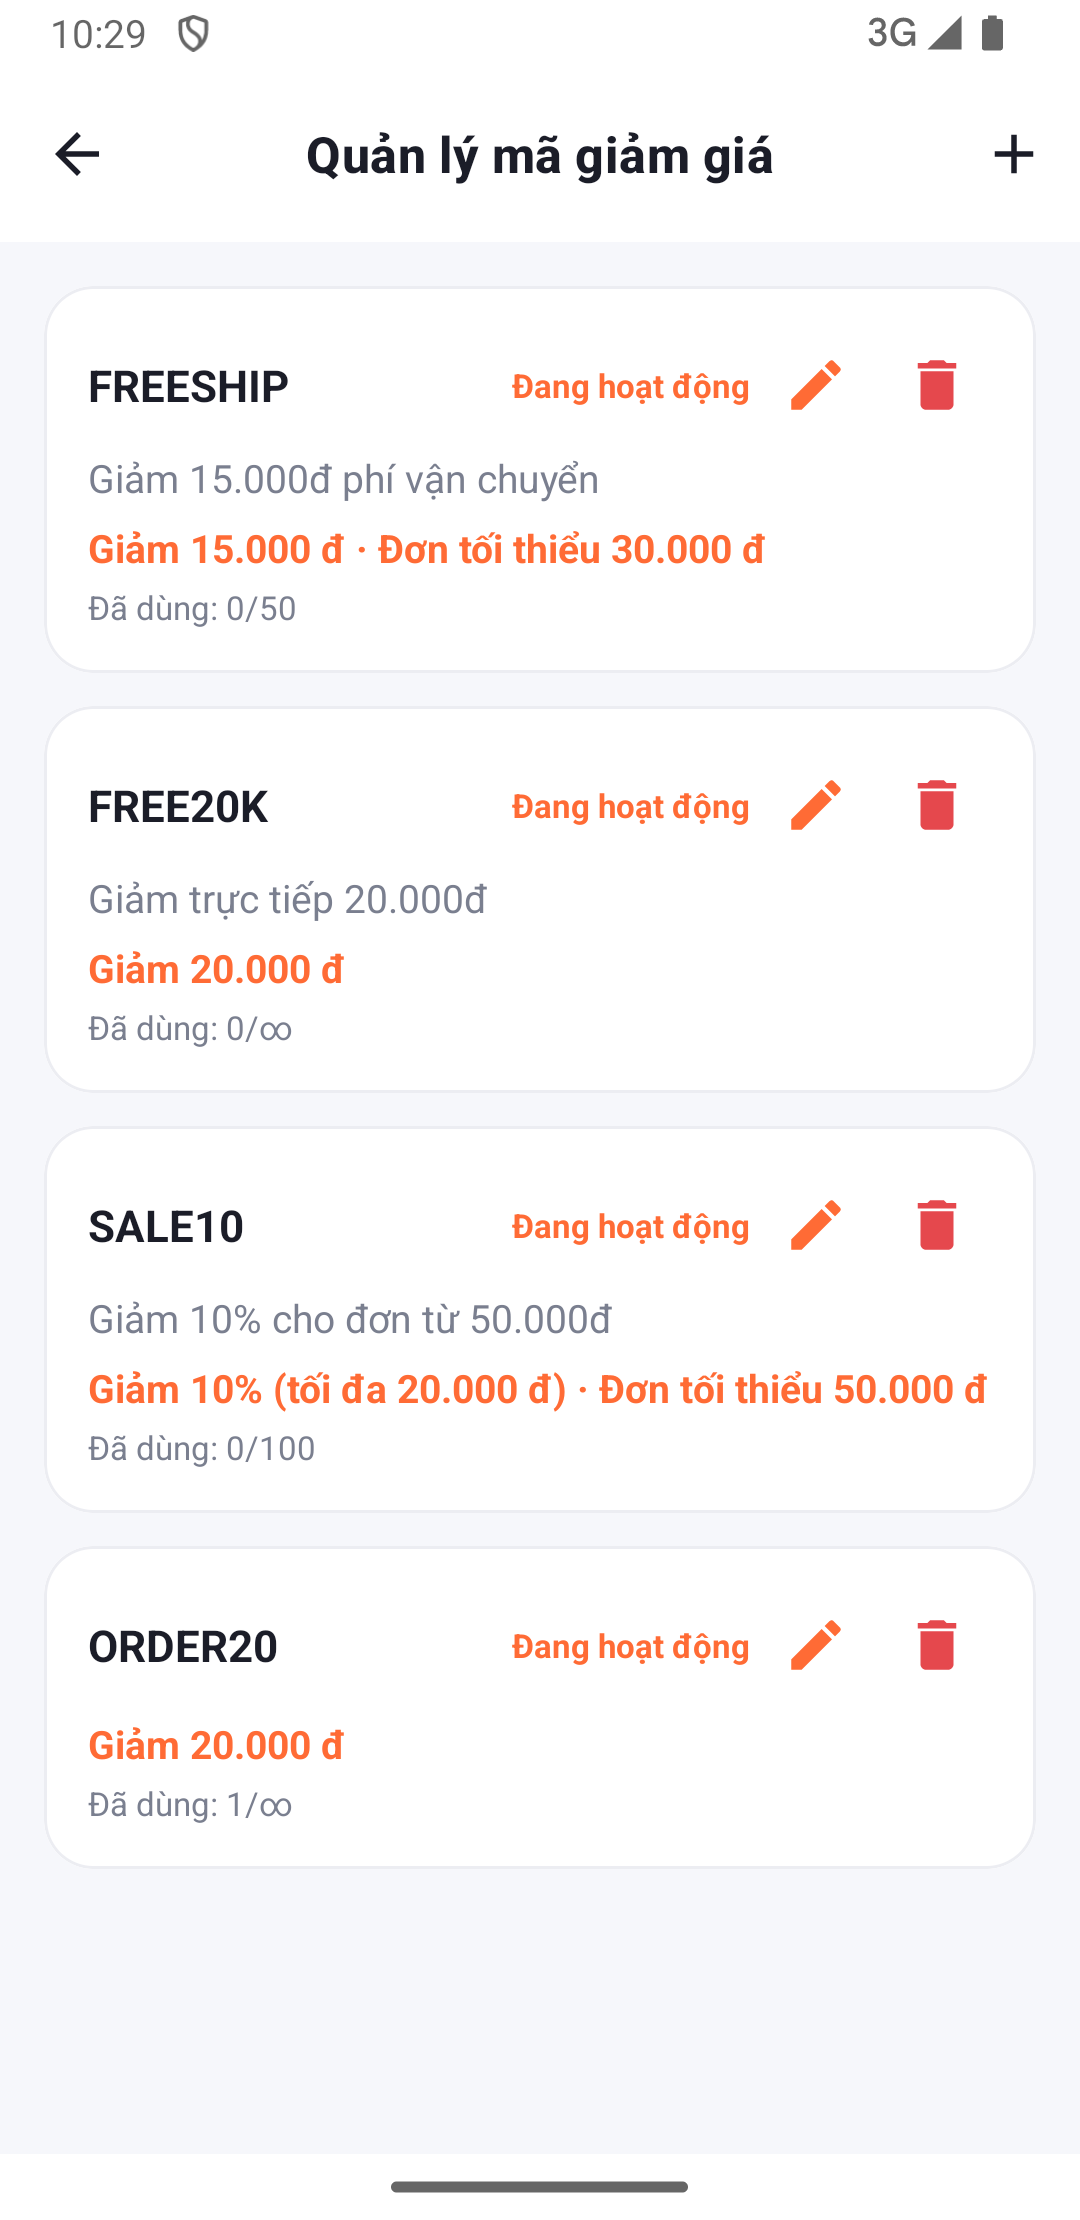
\includegraphics[width=0.75\textwidth]{images/admin_voucher.png}
\caption{Màn hình Quản lý mã giảm giá (Admin)}
\label{fig:admin-voucher}
\end{figure}

\begin{figure}[H]
\centering
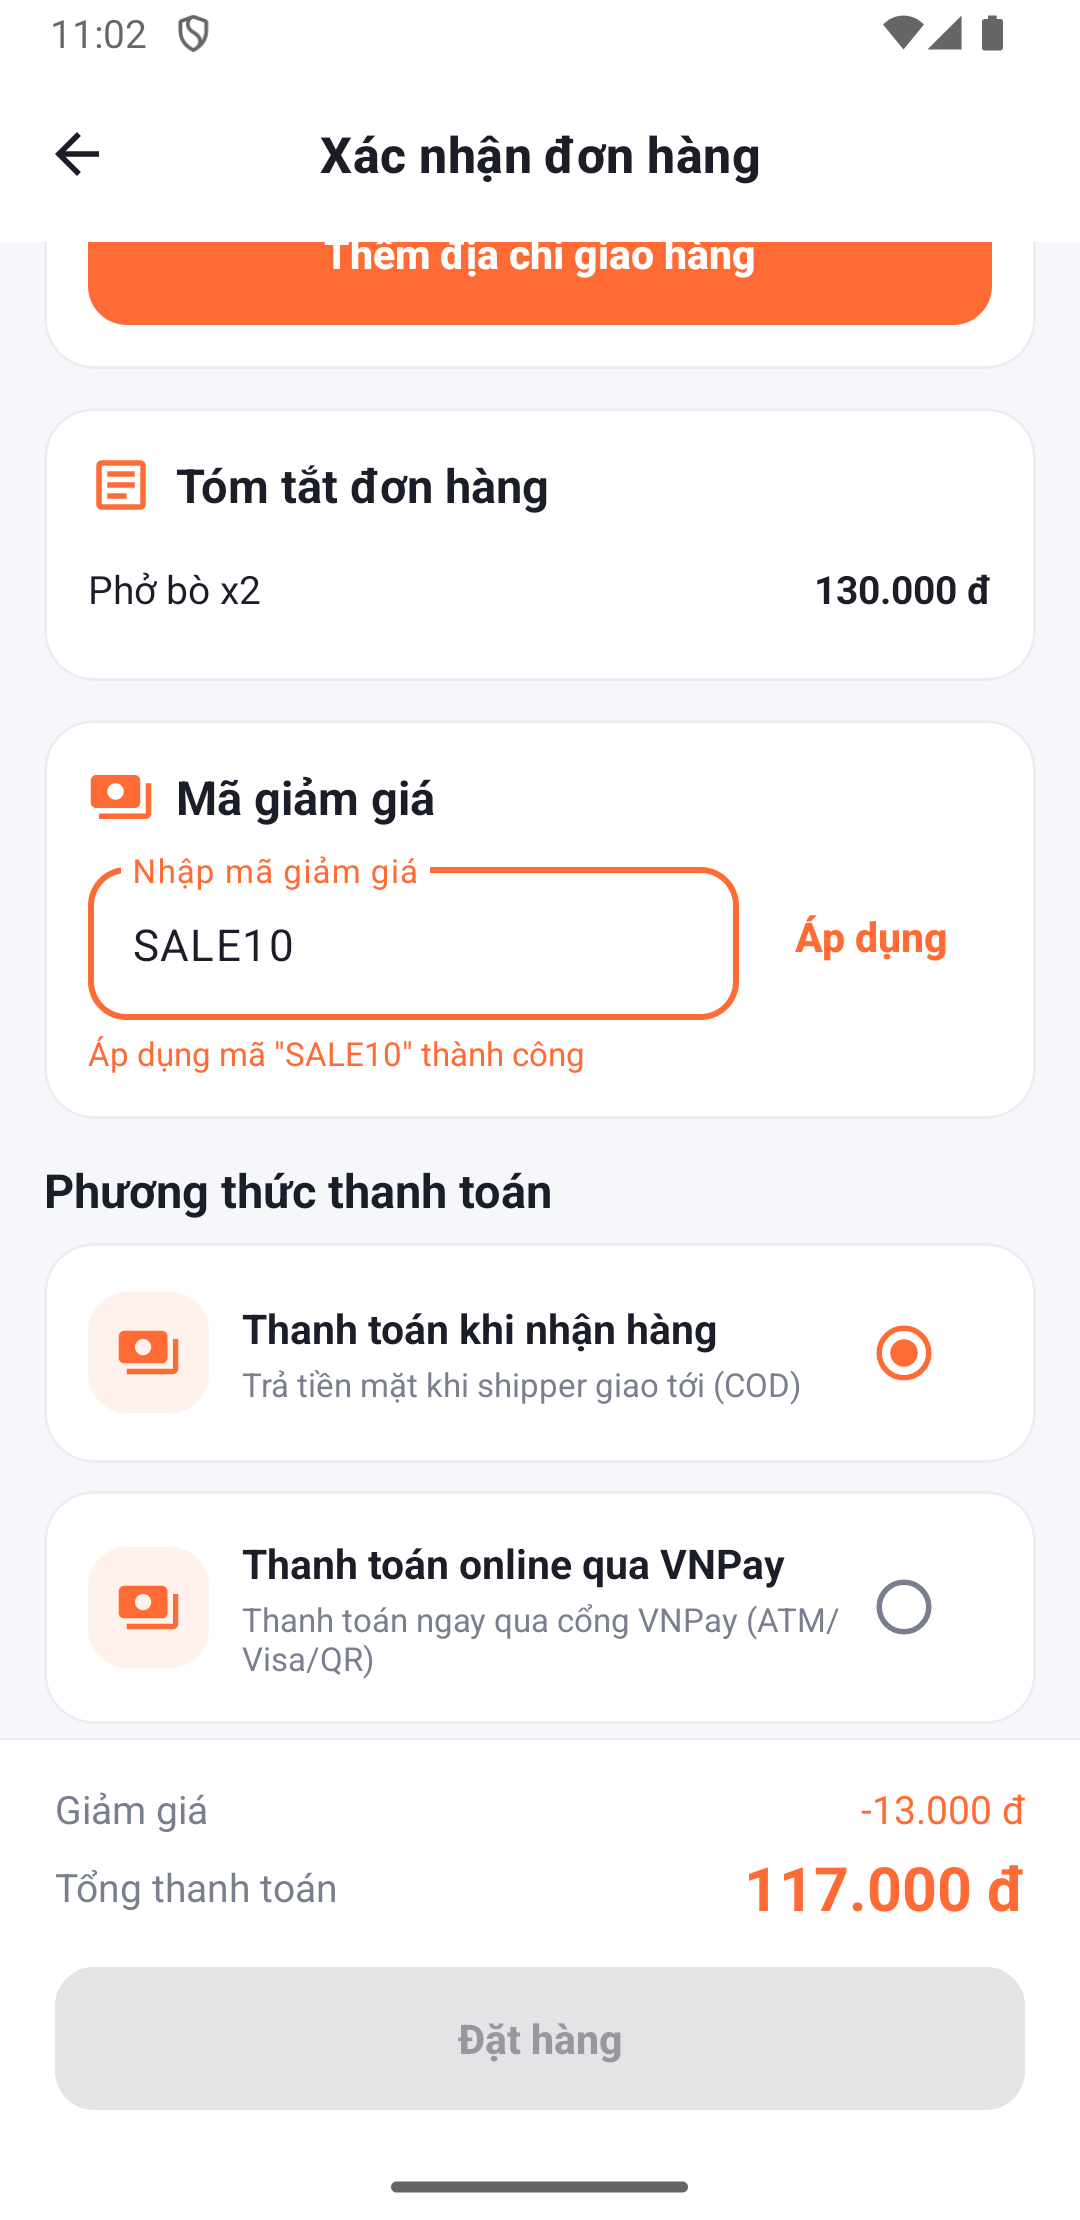
\includegraphics[width=0.75\textwidth]{images/checkout_voucher.png}
\caption{Màn hình Checkout -- áp dụng mã giảm giá (Khách hàng)}
\label{fig:checkout-voucher}
\end{figure}

% ===================================================================
\section{Kết luận và hướng phát triển}

\subsection{Kết quả đạt được}

Báo cáo đã trình bày việc phân tích, thiết kế và xây dựng hoàn chỉnh chức năng mã giảm giá cho hệ thống FoodGo, bao gồm: thiết kế cơ sở dữ liệu quan hệ, thiết kế và cài đặt API RESTful, cài đặt giao diện quản trị và giao diện khách hàng trên Android, và đặc biệt là giải quyết đúng đắn bài toán xử lý tương tranh khi nhiều yêu cầu cùng sử dụng một mã giảm giá có giới hạn số lượt dùng -- được kiểm chứng bằng test case thực nghiệm trên cơ sở dữ liệu thật.

\subsection{Hạn chế}

\begin{itemize}[leftmargin=*]
    \item Mỗi đơn hàng chỉ áp dụng được một mã giảm giá duy nhất (không hỗ trợ kết hợp nhiều mã).
    \item Chưa có thống kê hiệu quả sử dụng từng mã giảm giá cho quản trị viên (ví dụ tổng doanh thu đến từ các đơn có dùng mã).
\end{itemize}

\subsection{Hướng phát triển}

\begin{itemize}[leftmargin=*]
    \item Cho phép áp dụng đồng thời nhiều mã giảm giá không xung đột nhau.
    \item Gửi thông báo đẩy đến khách hàng khi có mã giảm giá mới phù hợp với lịch sử đặt hàng của họ.
    \item Tích hợp với chương trình tích điểm khách hàng thân thiết trong tương lai.
\end{itemize}

\end{document}
